
\clearpage
\part{Full Code breakdown by Function}
\section{main.py}
This script handles the creation of the UI as well as running the Maze Database, MazeGenerationNew and 
MazeRendererNew scripts.

\textcolor[RGB]{220,220,220}{\rule{\linewidth}{0.2pt}}
\begin{lstlisting}
def change_state(state):      

    des()
    if state == "start":    
        title = tk.Label(window, text = "\n Maze Game \n Version 2.0 \n", bg = "white", borderwidth=1, relief="groove").pack(fill = "x",pady=(250,20))
        enter_button = tk.Button(window, text = "Enter",bg = "white",width=30, command = lambda: change_state("username")).pack()
        exit_button = tk.Button(window, text = "Exit",width=30, bg = "white", fg = "red", command = lambda: exit()).pack(pady=3)
        if not installed:
            error_message = tk.Label(window,text="[PIL or Numpy not installed, PIL and Numpy are required for current version]",fg="red").pack(side="bottom",pady = 20)
    if state == "username": 
        title = tk.Label(window, text = "\n Accounts \n", bg = "white",  borderwidth=1, relief="groove").pack(fill = "x",pady=(20,100))
        top_seperator = tk.Canvas(window, height=50,width=0).pack()
        ...
\end{lstlisting}
The "change state" function takes the argument "state" and uses that to switch to a pre-defined set of UI elements, e.g. a main menu or a user select screen.

\begin{lstlisting}
def create_levels(lower,upper,number_of_columns,title,maze_type,completed):
    des()
    first = tk.Frame(window)
    first.pack(side='top')
    side = first
    title_ = tk.Label(window, text = ("\n" + title + "\nSelect a level\n"), bg = "white", borderwidth = 1, relief = "groove").pack(in_ = first,fill = "x",pady=20)
    top_seperator = tk.Canvas(window, height=50,width=0).pack(in_ = side)
    dict_one = {
                "normal":0,
                "diamond":1
                }
    for i in range((lower),(upper+1)):
            text = str(i)                          
            try:
                if completed[dict_one[maze_type]].count(text) > 0:
                    fg = "green"
                    text += "\n(Complete)"
                else:
                    fg = "black"
            except:
                fg = "black"
            button = tk.Button(window, text=text, width = 10, relief = 'groove', bg = "white",fg = fg)
            button.config(command = lambda mt = maze_type, btn = button : load_maze(lower,upper,title,mt,dict_one[maze_type],btn))
            button.pack(in_ = side, side = "left", padx=10,pady=10)
            if (i%number_of_columns) == 0:
                middle = tk.Frame(window)
                middle.pack(side = "top")
                side = middle
    back_button = tk.Button(window, text = "Back", command = lambda: change_state("maze select")).pack(side="bottom",pady=10)

\end{lstlisting}
"Create levels" generates a set of buttons with numbers on them, defined by the range entered in the parameters (lower and upper). If the level has already been completed by the user then the text will be green! It lays them out based on the parameter "number\_of\_columns".
When the user clicks on one of these buttons the actual button is passed to the function so that the text on the button can be properly read.

\clearpage

\begin{lstlisting}
def load_maze(lower,upper,title,maze_type,btn):   #Generates the maze and then passes the data along with other parameters to the MazeRenderer script
    maze_size = int((btn['text']).replace("\n(Complete)","")) + 3
    if installed:        
        maze_data = main(maze_size,maze_size,1000,maze_type)
        dict_two = {
            "normal":[[len(maze_data[0])-1],[0],[0,len(maze_data)-1]],
            "diamond":[[len(maze_data[0])-1],[0],[0,len(maze_data)-1]]
            }
        win_pos_x = (dict_two[maze_type])[0]
        win_pos_y = (dict_two[maze_type])[1]
        start_pos = (dict_two[maze_type])[2]
        dimensions = alter_screen()
        won = play_maze(dimensions[0],dimensions[1],(str(maze_size) + " x " + str(maze_size)),10,win_pos_x,win_pos_y,start_pos,maze_data)
    else:
        won = True  #Maze auto-completes if PIL is not installed
    if won:
        if user_id != 0:
            Db.add_completed_level(connection,maze_size-3, maze_type,user_id)
    completed = Db.get_list_of_completed_levels(connection,user_id)
    create_levels(lower,upper,4,title,maze_type,completed)

\end{lstlisting}
The main job of "Load Maze" is to translate the parameters entered pass them to the MazeGenerationNew, script take the generated
data and then pass that, along with other translated parameters, to the MazeRenderNew script.

\begin{lstlisting}
def custom_maze(maze_type,width,height,cube_size,title):    #Same as the function above but for custom mazes
        width = int(width.get())
        height = int(height.get())
        cube_size = int(cube_size.get())
        maze_data = main(width,height,1000,maze_type.get())
        dimensions = alter_screen()
        play_maze(dimensions[0],dimensions[1],(str(width) + " x " + str(height)),cube_size,[len(maze_data[0])-1],[0],[0,len(maze_data)-1],maze_data)
        change_state('custom maze',True)

\end{lstlisting}
"Custom Maze" is a version of "Load Maze" for cutom mazes with unsual heights and widths. An improvement to the code would be combining the two above functions.

\begin{lstlisting}
def set_user_id(username,guest):    #Sets the user ID
    global user_id
    if guest:
        user_id = 0
    else:
        user_id = username
    change_state("maze select")

\end{lstlisting}
"Set User ID" is a simple function that sets the global user\_id. The user\_id is used to retrieve data about the user from maze.db, if the user is a guest then the ID is set to 0
and all code involving the user\_id is skipped.

\begin{lstlisting}
def reset_progress():           #Resets the current users progress
    username = Db.delete_user(connection, user_id)
    Db.create_new_user(connection, username)
    change_state("maze select")
\end{lstlisting}
This functions is also simple. It resets the progress of the user by deleting the user from the and then creating them again, utilizing the below function.

\begin{lstlisting}
def new_user(user_entry_widget):    #Creates a new user named using the entered user name
    name = user_entry_widget.get()
    Db.create_new_user(connection,name)
    change_state("username")
\end{lstlisting}
Simply, adds a new entry to the database containing a new user.

\clearpage

\begin{lstlisting}
def des(): #Deletes all current widgets in "window"
    widget_list = all_children(window)
    for item in widget_list:
        item.pack_forget()
\end{lstlisting}
This function deletes all current widgets, this is used to reset the UI so that new UI can be made in its place. It utilizes the below function
which creates a list of all widgets pareneted to the entered object. The object entered in the case of "des()"  is the whole tkinter window.
\begin{lstlisting}
def all_children(window): # This makes a list of all the current widgets
    list_one = window.winfo_children()
    for item in list_one:
        if item.winfo_children() :
            list_one.extend(item.winfo_children())
    return list_one
\end{lstlisting}

\begin{lstlisting}
def alter_screen():     #Changes screen dimenions to make the rendering of the maze faster
    const = 2
    dimensions = [0,0]
    dimensions[0] = int(screen_width/const)
    dimensions[1] = int(screen_height/const)
    return dimensions
\end{lstlisting}
"Alter Screen" shrinks the size of the layers (images created in the renderer) to make the creation of said layers in the rendering section of the code easier
and less resource consuming.

%%%%%%%%%%%%%%%%%%%%%%%%%%

\clearpage
\section{MazeDatabase.py}
Script for interaction with the maze.db for storing users and completed levels, utilizes SQL.

\textcolor[RGB]{220,220,220}{\rule{\linewidth}{0.2pt}}
\begin{lstlisting}
def main_database():    #Creates the database (if it wasn't already created) and establishes a connection to it 
    user_table = " CREATE TABLE IF NOT EXISTS users (
id integer PRIMARY KEY,
username text NOT NULL
); "
    completed_levels_table = " CREATE TABLE IF NOT EXISTS completedLevels (
id integer PRIMARY KEY,
normal_maze text,
diamond_maze text,
user_id integer NOT NULL,
FOREIGN KEY (user_id) REFERENCES users (id)
); " 
    connection = create_connection(r"Maze.db")
    if connection is not None:
        create_table(connection,user_table)
        create_table(connection,completed_levels_table)
    else:
        print("Database Connection Error")
    return connection
\end{lstlisting}
This function is run to intialize the database, composed of two tables, (if it's not already created) and  establish a connection to said database.
The comment explaining the datbase is included below, along with a diagram.
\begin{lstlisting}
"DATABASES
Users table stores name and user_id + any additional information needed
CompletedLevels table stores the completed levels linked to the foreign key user_id and a primary key completed_id. There will be two columns, one for normal mazes, one for diamond mazes
the completed levels will be serialized as such (1#3#4#12...) and when the string is imported it will be split into a list."
\end{lstlisting}
\begin{center}
	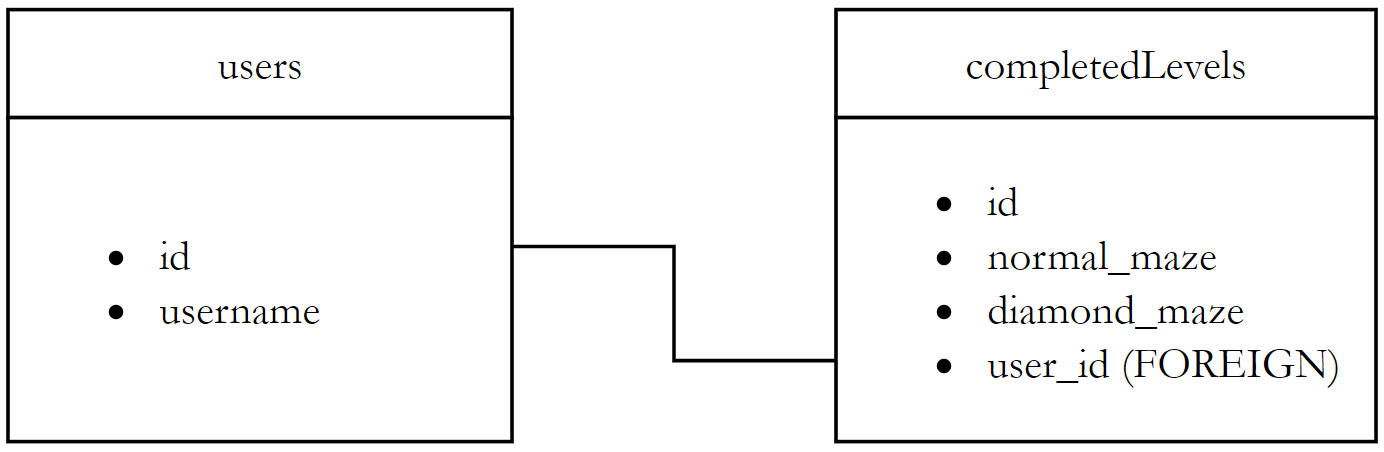
\includegraphics[scale=0.5]{Database Diagram}
\end{center}
\begin{lstlisting}
def create_new_user(connection, username):
    #Create the new user
    new_user_sql = "INSERT INTO users(username) VALUES(?)"
    cursor = connection.cursor()
    cursor.execute(new_user_sql, (username,))
    user_id = cursor.lastrowid
    connection.commit()
    #Then create the sibling entry in the CompletedLevels table based of the generated user_id
    new_completed_levels_sql = "INSERT INTO completedLevels(normal_maze, diamond_maze, user_id) VALUES(?,?,?)"
    cursor = connection.cursor()
    cursor.execute(new_completed_levels_sql, ("","",user_id))
    connection.commit()
\end{lstlisting}
"Create New User" inserts a row into the \textbf{users} table containing the entered username and then makes a sister entry in \textbf{completedLevels}. It uses
cursor.lastrowid to get the correct user id.
\clearpage
\begin{lstlisting}
def delete_user(connection, user_id):
    sql = 'SELECT username FROM users WHERE id = ?'
    cursor = connection.cursor()
    cursor.execute(sql, (user_id))
    result = cursor.fetchall()
    #Delete user entry
    sql = 'DELETE FROM users WHERE id=?'
    cursor = connection.cursor()
    cursor.execute(sql, (user_id))
    connection.commit()
    #Delete completedLevels entry
    sql = 'DELETE FROM completedLevels WHERE user_id=?'
    cursor = connection.cursor()
    cursor.execute(sql, (user_id))
    connection.commit()
    return result[0][0]
\end{lstlisting}
"Delete User" removes an entry from users and completedLevels based on the entered user\_id. It will also return the username from said user so that they can
be recreated in the "Reset Progress" function.

\begin{lstlisting}
def get_list_of_users(connection):
    user_list = []
    cursor = connection.cursor()
    cursor.execute("SELECT * FROM users")
    result = cursor.fetchall()
    for row in result:
        user_list.append((str(row)[1:-1]).split(','))
    return user_list
\end{lstlisting}
This function is implemented in "Change State" and is used when creating the buttons for the users in the user select screen. Contained within each
entry in the list is both the user\_id and the username.

\begin{lstlisting}
def add_completed_level(connection, level_number, maze_type, user_id):    #Uses the user id to alter the user's completed levels
    completed = get_list_of_completed_levels(connection, user_id)
    dict_one = {
                "normal":0,
                "diamond":1
                }
    formatted = ''
    for level_num in completed[dict_one[maze_type]]:
        print(level_num)
        formatted = formatted + level_num + "#"
    formatted = formatted + str(level_number)
    if maze_type == "normal":
        sql = "UPDATE completedLevels SET normal_maze = ? WHERE user_id = ?"
    elif maze_type == "diamond":
        sql = "UPDATE completedLevels SET diamond_maze = ? WHERE user_id = ?"
    cursor = connection.cursor()
    cursor.execute(sql,(formatted,user_id))
\end{lstlisting}
"Add Completed Level" takes the current completed levels list converts it to a string,  adds the entered level to the string and then inserts
it into the correct entry in the database. It finds the correct entry based off the maze type and user\_id.
\begin{lstlisting}
\end{lstlisting}
The below function is implemented in "Add Completed Level" to get the current completed levels for both maze types.
\begin{lstlisting}
def get_list_of_completed_levels(connection, user_id):
    maze_find_sql = "SELECT normal_maze, diamond_maze FROM completedLevels WHERE user_id = ?"
    cursor = connection.cursor()
    cursor.execute(maze_find_sql,(user_id))
    result = cursor.fetchall()
    return [(result[0][0]).split('#'),(result[0][1]).split('#')]
\end{lstlisting}
"Get List of Completed Levels" takes the string stored in the database for all maze types and converts them into a 2D array. 
The format for the string is explained in the comment explaning the database above.

\clearpage
\begin{lstlisting}
def create_connection(db_file):
    connection = None
    try:
        connection = sqlite3.connect(db_file)
    except Error as e:
        print(e)
    return connection
\end{lstlisting}

\begin{lstlisting}
def create_table(connection, create_table):
    try:
        cursor = connection.cursor()
        cursor.execute(create_table)
    except Error as e:
        print(e)
\end{lstlisting}
The above two functions are standard functions for interacting with a database. "Create Conncetion" creates a connection with a database file or creates the
database file and the establishes a connection with it if it doesn't already exist. The connection is then used the interact with the database itself. "Create Table"
actually would execute any SQL passed to it and acts more like an alias/simplification, however, it is only ever used to create tables.

%%%%%%%%%%%%%%%%%%%%%%%%%%

\clearpage
\section{MazeGenerationNew.py}
Uses Kruskal’s algorithm paired with a generated weight array to create the maze.

\textcolor[RGB]{220,220,220}{\rule{\linewidth}{0.2pt}}
\begin{lstlisting}
def intialize_array(width,height):
    #Intialize the array
    maze_array = []
    for x in range(0,width):
        maze_array.append([])
        for y in range(0,height):
            maze_array[x].append([1,1,1,1]) #Add a blank cell with all four walls to create an array that will be altered to generate a maze, this array is the data we return
    return maze_array
\end{lstlisting}
"Intialize Array" creates a 2D array formatted in the correct manner to be used as the \textbf{maze\_array} which represents the maze. This maze is made
up of cells, each cell being linked to a coordinate/index in the 2D array, with the cell being represented as a list of length four (i.e. [1,1,1,1]). Each number in
this list can be eithier a 1 or 0, representing a wall or empty space respectively. A diagram displaying this is placed below.
\begin{center}
	\fbox{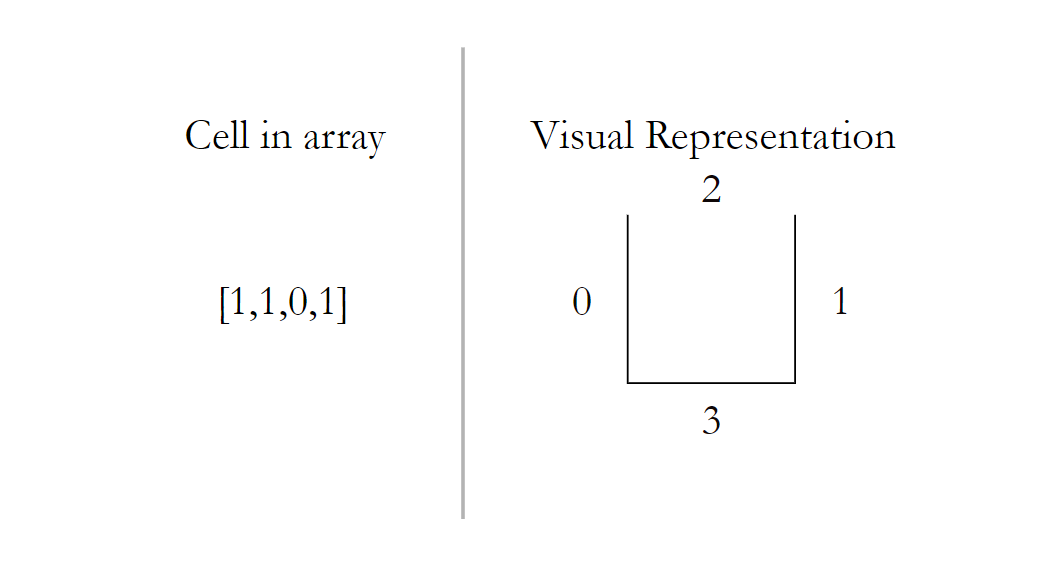
\includegraphics[scale=0.5]{Maze Cell Diagram}}

	\color{mygrey}(The numbers on the Visual Representation correlate to the index in the array)
\end{center}

\begin{lstlisting}
def generate_random_walls(height,width):    #Random walls for testing maze renderer
    #Intialize the array
    maze_array = []
    temp_list = [0,0,0,0,0,0,1]
    for x in range(0,width):
        maze_array.append([])
        for y in range(0,height):
            maze_array[x].append([random.choice(temp_list),random.choice(temp_list),random.choice(temp_list),random.choice(temp_list)])
    return maze_array
\end{lstlisting}
The above function is used only in testing, it can technically generate unbeatable mazes but due to the weighted chance to generate an empty or 
a wall (represented using temp\_list) it is unlikley. It  was mainly used in rendering testing but was also used when testing maze collision. 
\clearpage
\begin{lstlisting}
def kruskals_algorithim(weight_group_array,width,height,max_weight): #Based loosely on the algorithim as described in "Mazes for Programmers"
    maze_array = intialize_array(width,height)
    group_designation = 1                                                                                                                                           
    temp_list_empty = False
    while not all_in_one_group(weight_group_array,height,width) and not temp_list_empty: #Only ends loop when no new corridors can be checked and all the corriders are in the same group
        temp_list = lowest_values_pos(weight_group_array,width,height,max_weight+1)
        if temp_list == []:
            temp_list_empty = True
        else:
            dict_one = {
                0:[0,-1,1],
                1:[0,1,0],
                2:[-1,0,3],
                3:[1,0,2]
                }
            for pos in temp_list:
                can_connect = True
                difference = dict_one[pos[2]]
                current_pos_group = (weight_group_array[pos[0]][pos[1]])[4]                
                try:
                    if pos[0]+difference[0] == -1 or pos[1]+difference[1] == -1:
                        error = pos[100]
                    connected_pos_group = (weight_group_array[pos[0]+difference[0]][pos[1]+difference[1]])[4]
                    if current_pos_group == 0:
                        if connected_pos_group == 0:
                            (weight_group_array[pos[0]][pos[1]])[4] = group_designation
                            (weight_group_array[pos[0]+difference[0]][pos[1]+difference[1]])[4] = group_designation
                            group_designation += 1
                        else:
                            (weight_group_array[pos[0]][pos[1]])[4] = (weight_group_array[pos[0]+difference[0]][pos[1]+difference[1]])[4]
                    else:
                        if current_pos_group == connected_pos_group:
                            can_connect = False
                        elif connected_pos_group == 0:
                            (weight_group_array[pos[0]+difference[0]][pos[1]+difference[1]])[4] = current_pos_group
                        elif connected_pos_group != 0:
                            group_pos = get_all_in_group(weight_group_array,width,height,connected_pos_group)
                            for pos2 in group_pos:
                                (weight_group_array[pos2[0]][pos2[1]])[4] = current_pos_group
                    if(can_connect):
                        (maze_array[pos[0]][pos[1]])[pos[2]] = 0
                        (maze_array[pos[0]+difference[0]][pos[1]+difference[1]])[difference[2]] = 0
                    (weight_group_array[pos[0]][pos[1]])[pos[2]] = max_weight+2
                    (weight_group_array[pos[0]+difference[0]][pos[1]+difference[1]])[difference[2]] = max_weight+2
                except IndexError:
                    (weight_group_array[pos[0]][pos[1]])[pos[2]] = max_weight+2
                    if (weight_group_array[pos[0]][pos[1]])[4] == 0:
                        (weight_group_array[pos[0]][pos[1]])[4] = group_designation
                        group_designation += 1
    return maze_array
\end{lstlisting}
"Kruskals Algorithim" is the algorithim used to actually generate the mazes. It does this utilizing a \textbf{weight\_group\_array} and by altering
the corridors between cells in the \textbf{maze\_array}. The outline of how it works is this; All cells have a group, at the start this is the default group (i.e. zero).
Any cell within a group is reachable by any other cell in a group (unless it is the default group), they are essentially perfect mazes within the larger maze.
At the start of each iteration of the while loop the code finds corridors (connections between cells) based on the lowest weight, this is done using the afformentioned
\textbf{weight\_group\_array} and the function below.
\clearpage
\begin{lstlisting}
def lowest_values_pos(wg_array,width,height,compared_to):   #Finds all the connections in the maze with the lowest weight value
    temp_list = []
    for x in range(0,width):
        for y in range(0,height):
            for i in range(0,4):
                if wg_array[x][y][i] < compared_to:
                    compared_to = wg_array[x][y][i]
                    temp_list = []
                    temp_list.append([x,y,i])
                elif wg_array[x][y][i] == compared_to:
                    temp_list.append([x,y,i])
    return temp_list
\end{lstlisting}
The actual \textbf{weight\_group\_array} or\textbf{wg\_array}  is generated by functions "Generate Walled Maze" and "Generate Diamond Maze" discussed lower down.
Once a corridor is chosen an actual connection is attempted, a connection will only not be made if, 1. The connection is being made to an area outside the maze or 2. The
connection is being made to a cell that is already in the same group as the chosen cell. The latter of the two fail states exists so that the generation doesn't remove every single wall.
If a connection is made between two cells with non-default but different groups then all cells in the group that doesn't contain the chosen cell are changed to be in the group
with the chosen cell. This process is done using "Get All In Group" (shown below).
\begin{lstlisting}
def get_all_in_group(wg_array,width,height,group):  #Gets the positions of all the cells that have the group specified
    temp_array = []
    for x in range(0,width):
        for y in range(0,height):
            if (wg_array[x][y])[4] == group:
                temp_array.append([x,y])
    return temp_array
\end{lstlisting}
The algorithim will run untill all cells are in the same group (and that group is not the default) meaning any cell within the maze can be reached from any other cell. To check
that all cells are in the same group the function "All In One Group" is used.
\begin{lstlisting}
def all_in_one_group(wg_array,height,width):    #Checks to see if every cell is in a singular group (a.k.a every cell can be reached from any other cell)
    returned = True
    first_group = "null"
    for x in range(0,width):
        for y in range(0,height):
            temp = (wg_array[x][y])[4]
            if first_group == "null":
                first_group = temp
            if temp != first_group or temp == 0:
                returned = False                
    return returned
\end{lstlisting}
\begin{lstlisting}
def generate_walled_maze(width,height,max_weight):
    weight_group_array = []                 
    for x in range(0,width):
        weight_group_array.append([])
        for y in range(0,height):
            weight_group_array[x].append([random.randint(1,max_weight),random.randint(1,max_weight),random.randint(1,max_weight),random.randint(1,max_weight),0])   #Create a "sister" array that stores the weight values and group of each cell
    maze_array = kruskals_algorithim(weight_group_array,width,height,max_weight)    #Use the weight array to generate an actual maze
    return maze_array
\end{lstlisting}
"Generate Walled Maze" generates a simple \textbf{weight\_group\_array} by randomly generating weight values for each cell.
\clearpage
\begin{lstlisting}
def generate_diamond_maze(width,height,max_weight):
    weight_group_array = []
    for x in range(0,width):
        weight_group_array.append([])
        for y in range(0,height):
            weight_group_array[x].append([random.randint(1,max_weight),random.randint(1,max_weight),random.randint(1,max_weight),random.randint(1,max_weight),0])
    #Manipulate the weight group array to make the algorithim generate a diamond maze with random gaps in the walls
    center_of_maze = [int(width/2),int(height/2)]
    pos_to_change = center_of_maze
    counter = 1
    circling = True
    translate_to_displacement = {
        1:[0,1],
        2:[1,0],
        3:[0,-1],
        0:[-1,0]
        }
    translate_to_wall_index = {
        1:2,
        2:1,
        3:3,
        0:0
        }
    while circling:
        modded_counter = counter % 4
        displacement = translate_to_displacement[modded_counter]
        wall_index = int(translate_to_wall_index[modded_counter])
        length_counter = counter // 2 + (counter % 2)
        for i in range(1,length_counter):
            #Check to see if current cell is within maze
            if pos_to_change[0] > width-1 or pos_to_change[1] > height-1:
                pass
            else:
                #If it is then remove the wall leading to the new cell
                weight_group_array[pos_to_change[0]][pos_to_change[1]][wall_index] = counter
            #Move into the new cell
            pos_to_change = [pos_to_change[0]+displacement[0],pos_to_change[1]+displacement[1]]
        counter += 1
        #Fail state check
        if pos_to_change[0] > width and pos_to_change[1] > height:
            circling = False
    weight_group_array[center_of_maze[0]][center_of_maze[1]] = [0,0,0,0,0] #Remove all walls from center
    maze_array = kruskals_algorithim(weight_group_array,width,height,max_weight)
    return maze_array 
\end{lstlisting}
"Generate Diamond Maze" is a more complicated  \textbf{weight\_group\_array} generator used to create a maze with an actual texture. It does this by
circling from cells from the maze center changing the weights so that the corridors are created in a certain way leading to a pyramid/diamond pattern. This method
could also be used to create a circular maze, however, that type of maze is significatly less fun to play. 

%%%%%%%%%%%%%%%%%%%%%%%%%%

\clearpage
\section{Window.py}
Uses tkinter, NumPy and pillow (a fork of PIL (Python Imaging Library)) to create layered editable images on screen. Using tkinter it also handles input, unfortunately the window needs to be clicked on for input to be registered.

\textcolor[RGB]{220,220,220}{\rule{\linewidth}{0.2pt}}
\begin{lstlisting}
class Window():
    pixel_scale = 1
    last_key_pressed = None
    
    def __init__(self, height, width, default_colour, title):   #Creates the intial image and sets intial values
        self.height = int(height)
        self.width = int(width)
        self.title = title
        self.default_colour = default_colour
        self.window = create_tkinter_window(self.height, self.width, self.title)
        self.screen = create_canvas(self.window)
        self.layers = []
        self.layers.append(self.Layer(self,self.height,self.width,self.default_colour)) #Create the background layer
\end{lstlisting}
Above is the "Window" class and its "\_\_init\_\_" function. A "Window" instance has a tkinter window (with a canvas called .screen) upon which
layers can be placed. In the "\_\_init\_\_" function only a background/default layer is created. Each layer is also an instance of
a class called "Layer", which is a sub-class of "Window". However, it being a sub-class doesn't actually mean anything (other than making it easier to
understand what "Layer" is meant for) so .layers is needed in "Window" to store that given window's layers. The code for "Layer" is shown below:
\begin{lstlisting}
    class Layer():  #Layer Objects

        def __init__(self,window,height,width,default_colour):
            self.height = height
            self.width = width
            self.default_colour = default_colour
            self.layer_num = len(window.layers)
            self.array = create_image_array(height,width,default_colour)
            self.generated_image = ImageTk.PhotoImage(master = window.screen,image=Image.fromarray(self.array))
            self.image = window.screen.create_image(width,height,image=self.generated_image)
\end{lstlisting}
Layers are used as a form of optimisation so that when we update the screen, to move the player for example, we only need
to update a very small image rather than the whole maze image. 
\begin{lstlisting}
    def move_layer(self,new_coords,layer_num = 0):  #Moves a layer to a given position
        #Get Current Top Left of layer Coords
        old_coords = self.screen.coords(self.layers[layer_num].image)
        old_coords[0] = old_coords[0] - (self.layers[layer_num].height/2)
        old_coords[1] = old_coords[1] - (self.layers[layer_num].width/2)
        #Move to new position
        self.screen.move(self.layers[layer_num].image,new_coords[0] - old_coords[0],new_coords[1] - old_coords[1])
\end{lstlisting}
"Move Layer" is moves any given layer to entered coordinates. While there is a standard move function for image objects on
tkinter canvases, it moves objects by a 2D Vector rather than being coordinate based.
\begin{lstlisting}
    def delete_layer(self,layer):
        self.screen.delete(self.layers[layer].image)
        self.layers.pop(layer) 
\end{lstlisting}
"Delete Layer" deletes a layer by first removing its image from the canvas and then poping it from the .layers list. Unlike other functions
that interact with layers this one requires a layer number to be entered (whereas others have a default of the background layer) so that
the background layer isn't deleted by mistake. 
\begin{lstlisting}
    def reset(self, layer_num = 0):    #Resets the entered layer, used so the line below doesn't need to be typed everytime
        self.layers[layer_num].array = create_image_array(self.layers[layer_num].height,self.layers[layer_num].width,self.layers[layer_num].default_colour)
\end{lstlisting}
There is also "Reset" which will just reset a layer (based of the "Window" object .default\_colour) rather than deleting it.
\begin{lstlisting}
    def set_pixel(self, coords, colour, layer_num=0): #Change a pixel in the image array
        coords[0] = (coords[0] * self.pixel_scale) - (self.pixel_scale - 1)
        coords[1] = (coords[1] * self.pixel_scale) - (self.pixel_scale - 1)
        for x in range(coords[0],coords[0]+self.pixel_scale):
            for y in range(coords[1],coords[1]+self.pixel_scale):
                try:
                    self.layers[layer_num].array[y,x] = colour
                except IndexError:
                    pass   
\end{lstlisting}
"Set Pixel" allows any pixel on the entered layer to be altered based off the coordinates entered, a range of pixels can also be affected 
if the pixel scale isn't one. It does this by altering the coresponding index in a numpy array, this numpy array is then converted into an
image using Pillow (PIL) and then subsequently turned into an image tkinter will accept, also using PIL. The image conversion is all done
in the "Update" function, alongside updating the tkinter window itself.
\begin{lstlisting}
    def update(self, layer_num = 0):   #Updates an entered layer
        try:
            self.layers[layer_num].generated_image = ImageTk.PhotoImage(master = self.screen,image=Image.fromarray(self.layers[layer_num].array)) #Generate a updated image from the image array
            self.screen.itemconfig(self.layers[layer_num].image, image = self.layers[layer_num].generated_image)    #Applies the generated image
        except IndexError:
            print("Invalid Layer")
        self.window.update()
\end{lstlisting}
\begin{lstlisting}
    def init_input(self):                   #Input created using tkinter, last key pressed = key pressed that frame
        def on_key_press(event):
            self.last_key_pressed = event.char
            if self.last_key_pressed == '\boxempty':
                self.last_key_pressed = 'esc'
        def on_key_up(event):
            self.last_key_pressed = None
        self.window.bind('<KeyPress>', on_key_press)
        self.window.bind('<KeyRelease>', on_key_up)
\end{lstlisting}
The "Window" class also handles input, utilizing tkinter's event system. "Init Input" must be run to start input and within the function two other
functions are also defined. "On Key Press" sets .last\_key\_pressed to the current key being pressed when a key is being pressed (as indicated by tkinter), while
"On Key Up" sets .last\_key\_pressed back to \textcolor{amber}{None}. 
\begin{lstlisting}
    def set_fullscreen(self, boolean):  #Turns fullscreen on and off based on boolean
        self.window.overrideredirect(True)
        self.window.overrideredirect(False)
        self.window.attributes('-fullscreen',boolean)
        self.screen.pack(fill="both", expand=True)

    def set_pixel_scale(self, num): #Used to change the pixel scale
        self.pixel_scale = num

    def quit(self):                             #Quits window
        for i in range(0,len(self.layers)):
            self.reset(i)
        self.window.destroy()
        del self
\end{lstlisting}
"Set Fullscreen", "Set Pixel Scale" and "Quit" are the three functions in the "Window" class that don't directly interact with a certain layer. "Set Fullscreen" allows for fullscreen
to be toggled on and off based on the parameter "boolean", "Set Pixel Scale" allows for the pixel scale to be changed in a less akward manner and "Quit" simply deletes every layer,
destroys the tkinter window and then does the same to the instance of the class.

\begin{lstlisting}
def create_tkinter_window(height, width, title):    #Creates a tkinter window
    window = tk.Tk()
    window.title(title)
    window.geometry(str(width) + "x" + str(height))
    #window.overrideredirect(1) #Removes the Titlebar
    return window
\end{lstlisting}
"Create Tkinter Window" and the two other final functions in "Window.py" aren't directly related to the "Window" class but are used within it. "Create Tkinter Window" simply creates
a tkinter window based of the parameters entered and then returns said window.
\begin{lstlisting}
def create_canvas(tkinter_window):  #Creates a tkinter canvas
    canvas = tk.Canvas(tkinter_window, bg="black")
    canvas.pack(fill="both",expand=True)
    return canvas
\end{lstlisting}
"Create Canvas" adds a canvas object to the passed tkinter window, the canvas is then made to fill the entire window. The canvas object it also returned.
\begin{lstlisting}
def create_image_array(height,width,colour): #Creates the intial image array
    image_array = np.zeros([height+1,width+1,3],dtype=np.uint8)
    image_array.fill(colour)
    return image_array
\end{lstlisting}
"Create Image Array" makes a numpy array and then fills it with the desired greyscale colour, entered as any value between 0 and 255, finnally the new image
array is returned.
%%%%%%%%%%%%%%%%%%%%%%%%%%

\clearpage
\section{MazeRendererNew.py}
Used when actually playing a maze, mainly used to implement the Window.py script to correctly draw the maze but also handles collision detection and a check to see if the player has won.

\textcolor[RGB]{220,220,220}{\rule{\linewidth}{0.2pt}}
\\
\begin{lstlisting}
\end{lstlisting}
"Play Maze" is the longest function in my entire NEA totaling around 130 lines of code, hence I'll explain it section by section rather than all at once.
\begin{lstlisting}
def play_maze(width,height,title,cube_size,win_pos_x,win_pos_y,start_pos,maze_data):
    #A cube_size of two and below will cause the squares to be too small to be properly represented properly on any pixelated screen, hence, 3 is the lowest the function allows
    if cube_size < 3: cube_size = 3 
    screen = Window.Window(height,width,0,"Test Window")
    screen.set_fullscreen(True)
    screen.init_input()
    screen.update()
    temp = 0 #Temporary Variable to manage progress of stand-in progress bar
    delta_time = 0
    fps = 0
    time_to_close = 1.5
    add_to_y = 0
    add_to_x = 0
    loading = True
    first_frame = True
    running = True
    position_set_to = [1,0]
    move_dir = ""
    player_pos = start_pos
    active_last_frame = True
    check_walls = True
    to_return = False
    ending = True
    drawing_per_frame = False
    input_confirmed = False
    input_delay = 0
\end{lstlisting}
Above is the section of play maze where every variable is set to it's starting value and the game window is intialized.

\begin{lstlisting}
    while running:
        #Anything in this loop is run every frame
        start_time = time.time() #For measuring execution time, it is used for debug, testing program speed and the calculation of delta_time        
\end{lstlisting}
The code above is short but essential. Everything executed whithin the while loop is run every frame and the start\_time variable is essential for calculations to be the same across systems with different frame rates.

\clearpage
\begin{lstlisting}
        #Input
        if input_delay <= 0:
            if screen.last_key_pressed != None and input_confirmed:
                if screen.last_key_pressed == 'esc':
                    running = False
                if screen.last_key_pressed == 'a':
                    add_to_x = -1
                    move_dir = "left"
                elif screen.last_key_pressed == 'd':
                    add_to_x = 1
                    move_dir = "right"
                elif screen.last_key_pressed == 'w':
                    add_to_y = -1
                    move_dir = "up"
                elif screen.last_key_pressed == 's':
                    add_to_y = 1
                    move_dir = "down"
                else:
                    move_dir = ""
                #Checks to make sure player can't go outside the maze
                if position_set_to[0] + add_to_x < 0 or position_set_to[0] + add_to_x > len(maze_data[0])-1:
                    add_to_x = 0
                    check_walls = False
                if position_set_to[1] + add_to_y < 0 or position_set_to[1] + add_to_y > len(maze_data)-1:
                    add_to_y = 0
                    check_walls = False
                #Checks to see if there is a wall in the players way
                if(wall(maze_data,[position_set_to[0] + add_to_x,position_set_to[1] + add_to_y],player_pos,move_dir)) and check_walls:
                    add_to_y = 0
                    add_to_x = 0
                check_walls = True
                input_confirmed = False
            else:
                position_set_to = player_pos
                add_to_y = 0
                add_to_x = 0
                input_confirmed = True
                input_delay = 0.1        #The time between moves
        else:
            input_delay -= delta_time
\end{lstlisting}
Above is the input code that is run each frame, first checks are run to see if any of the keys that have movements tied to them are pressed, if that is the case then it is checked to see if the move is legal (i.e. not through a wall or to somewhere outside the maze). Input delay is also managed here to make sure the player doesn't fully overshoot where they want to go.

\begin{lstlisting}
        #Game Code
        if debug:
            print(str(round((time.time() - start_time)*1000,1)) + "ms") #Prints execution time (per frame) to console
            print(temp)
\end{lstlisting}
Next is the start of the actual game code but first a check is run to see if debug mode is enabled. If it is then some information is printed to the console.

\begin{lstlisting}
        if loading:
            if temp >= 1:
                loading = False
                screen.reset()
            else:
                if temp == 0:
                    #Create Title
                    text("Maze Game",10,[0,-height/4],white,screen,[width,height])
                    time.sleep(0.1)
                progress_bar(width/2,temp,screen,[0,height/4],[width,height])  
                temp += 1 * delta_time    
\end{lstlisting}
If the game is still loading then this code is run every frame, it manages the loading bar and the large title.

\clearpage
\begin{lstlisting}
        elif not loading:                                               
            if first_frame == True:                
                first_frame = False            
                maze_width = (len(maze_data) * (cube_size-1))+1
                maze_height = (len(maze_data[0]) * (cube_size-1))+1
                if drawing_per_frame:
                    x = 0
                    y = 0
                else:
                    draw_maze([maze_height,maze_width],[width,height], cube_size,[win_pos_x,win_pos_y], screen, maze_data)
                #Create Maze Title
                text(title,3,[0,-((((len(maze_data) * (cube_size-1))+1)/2)+15)],white,screen,[width,height])
                #Instantiate Player
                player_pos = draw_player(True,cube_size,screen,player_pos,maze_width,maze_height,[width,height])  
                position_set_to = player_pos
\end{lstlisting}
Once the game has finshed loading on the first frame all of the following code is run. This includes setting variables to defaults, drawing the maze, title and player (utilizing functions detailed below).

\clearpage
\begin{lstlisting}
            else:
                if won(player_pos,win_pos_x,win_pos_y):#[len(maze_data[0])-1,0]):
                    if ending:
                        time.sleep(0.4) #Halts the game for a very short amount of time to make the transition to the end screen feel less abrupt
                        screen.delete_layer(1) 
                        screen.reset()                    
                        text("Maze Completed",10,[0,0],white,screen,[width,height])
                        text("#",5,[0,-50],white,screen,[width,height])
                        ending = False
                    if time_to_close < 0:
                        to_return = True
                        running = False
                    else:
                        time_to_close -= delta_time
                else:
                    if drawing_per_frame:
                        draw_maze_per_cell([maze_height,maze_width], [x,y], [width,height], cube_size, [win_pos_x,win_pos_y], screen, maze_data)
                        x += 1
                        if x == len(maze_data[y]):
                            x = 0
                            y += 1
                        if y == len(maze_data):
                            drawing_per_frame = False                  
                    player_pos = draw_player(False,cube_size,screen,[player_pos[0]+add_to_x,player_pos[1]+add_to_y],maze_width,maze_height,[width,height])
                    screen.update(layer_num = 1)
        delta_time = time.time() - start_time #delta_time is the time the program took to execute the last frame
\end{lstlisting}
After the first frame the following code is run every frame. First it checks to see if the player is in the winning position (utilizing a function also detailed below) and if they are all the apropriate code is run. Otherwise, if you are drawing per frame then the maze is drawn per frame, till the process is finished, and the players position is updated (currently the player isn't stopped from moving while the maze is drawn, however, that would be a very easy fix). Finally, delta\_time is updated so it can be used in the following frame.

\begin{lstlisting}
        try:
            fps = 1/delta_time         
        except:
            fps = '#'
    screen.quit()
    return to_return
\end{lstlisting}
At the very end of the function the fps calculation is run, however, the last two lines are only run when the while loop has been broken. The first closes the window and the second returns whether the player won or not.

\begin{lstlisting}
#CHECKS
def won(player_pos,win_pos_x,win_pos_y): #Compares player position to entered position
    if player_pos[0] in win_pos_x and player_pos[1] in win_pos_y:
        return True
    else:
        return False

def wall(maze_data,position_to_set_to,player_pos,move_dir): #Checks to see if there is a wall blocking the players way when they attempt to move
    if move_dir == "":
        return True
    dict_one = {
        "left":[0,1],
        "right":[1,0],
        "up":[2,3],
        "down":[3,2]
        }
    if (maze_data[player_pos[1]][player_pos[0]])[(dict_one[move_dir])[0]] == 1 or (maze_data[position_to_set_to[1]][position_to_set_to[0]])[(dict_one[move_dir])[1]] == 1:
        return True
    else:
        return False
\end{lstlisting}
The above two functions are used for checks, the former checks to see if the player position matches the winning position and the latter checks to see if there is a wall in the players way.

\begin{lstlisting}
#RENDERING
def draw_maze_per_cell(maze_dimensions, coords_to_draw, window_dimensions, cube_size, win_pos, screen, maze_data):  #Draw maze cell per frame
    offsetx = coords_to_draw[0] * (cube_size-1)
    offsety = coords_to_draw[1] * (cube_size-1)
    draw_rectangle([(0-(maze_dimensions[0]/2)+offsetx),((0-maze_dimensions[1]/2)+offsety)],cube_size,cube_size,False,white,screen,window_dimensions,0,maze_data[coords_to_draw[1]][coords_to_draw[0]])
    if won([coords_to_draw[0],coords_to_draw[1]],win_pos[0],win_pos[1]):
        draw_rectangle([(0-(maze_dimensions[0]/2)+offsetx+2),((0-maze_dimensions[1]/2)+offsety+2)],cube_size-4,cube_size-4,True,green,screen,window_dimensions,0)

def draw_maze(maze_dimensions, window_dimensions, cube_size, win_pos, screen, maze_data):   #Draw maze all at once
    offsetx = 0
    offsety = 0
    for y in range(0,len(maze_data)):
        for x in range(0,len(maze_data[y])):
            draw_rectangle([(0-(maze_dimensions[0]/2)+offsetx),((0-maze_dimensions[1]/2)+offsety)],cube_size,cube_size,False,white,screen,window_dimensions,0,maze_data[y][x])
            if won([x,y],win_pos[0],win_pos[1]):
                draw_rectangle([(0-(maze_dimensions[0]/2)+offsetx+2),((0-maze_dimensions[1]/2)+offsety+2)],cube_size-4,cube_size-4,True,green,screen,window_dimensions,0)
            offsetx += cube_size-1
        offsety += cube_size-1
        offsetx = 0
    screen.update() 
\end{lstlisting}
The functions above are both used to draw the maze, however, one draws a specific cell of the maze (utilized when drawing the maze frame by frame) while the second draws the maze all at once.

\begin{lstlisting}
def draw_player(first_pos,cube_size,screen,position,maze_width,maze_height,window_dimensions): #Draws the player in the center of a square, indicated by x and y coordinates
    player_size = (cube_size * 0.6)-1
    if first_pos:
        screen.layers.append(screen.Layer(screen,int(player_size),int(player_size),255))
    #Move the layer to the correct position
    new_pos = find_center_of_square(maze_width,maze_height,cube_size,position)
    new_pos[0] = int(window_dimensions[0]) + new_pos[0] 
    new_pos[1] = int(window_dimensions[1]) + new_pos[1]
    screen.move_layer(new_pos,layer_num=1)
    return position
\end{lstlisting}
"Draw Player" is used both to instantiate the player and/or move them. Most of this involves converting maze coordinates into screen space pixel measurments. 

\begin{lstlisting}
def progress_bar(width,progress,screen,offset,window_dimensions): #Generates a progress bar in the center of the screen, however, it's position can be shifted using the offset
    center = [0+offset[0],0+offset[1]]
    #Draw progress bar shell
    draw_rectangle([int(center[0]-width/2),center[1]],width,15,False,white,screen,window_dimensions,0,1)
    #Draw actual progress
    draw_rectangle([int(center[0]-width/2)+2,center[1]+2],int((width-4)*progress),11,True,white,screen,window_dimensions,0)
    screen.update()
\end{lstlisting}
"Progress Bar" can draw a progress bar with a specific amount of the bar filled. This is defined by the argument "progress". It naturally is drawn in the center of the screen but there is a offset function that allows it to be placed anywhere.

\begin{lstlisting}
def text(text,text_size,offset,colour,screen,window_dimensions,layer_num = 0):        #Draws entered text on screen in the font defined in 'font.txt', by default it is drawn in the center, however, this can be altered by entering an offset
    text_dict = {                                                       
        "a":0,"A":0,"b":1,"B":1,"c":2,"C":2,"d":3,"D":3,"e":4,"E":4,
        "f":5,"F":5,"g":6,"G":6,"h":7,"H":7,"i":8,"I":8,"j":9,"J":9,
        "k":10,"K":10,"l":11,"L":11,"m":12,"M":12,"n":13,"N":13,"o":14,"O":14,
        "p":15,"P":15,"q":16,"Q":16,"r":17,"R":17,"s":18,"S":18,"t":19,"T":19,
        "u":20,"U":20,"v":21,"V":21,"w":22,"W":22,"x":23,"X":23,"y":24,"Y":24,
        "z":25,"Z":25," ":26,"1":27,"2":28,"3":29,"4":30,"5":31,"6":32,"7":33,
        "8":34,"9":35,"0":36,"#":37
        }   #Maps a line in the text file to a character
    text_list = split(text)
    text_width = 0
    text_height = 5 * text_size
    offsetx = 0
    offsety = 0
    offset_character = 0
    for i in text_list:
        character_data = split_int(font[text_dict[i]])
        text_width += (int((len(character_data)*text_size)/5) + (1*text_size))
    for i in text_list:
        character_data = split_int(font[text_dict[i]])
        for y in range(0,5):
            for x in range(0,int(len(character_data)/5)):
                if character_data[(y*int(len(character_data)/5))+x] == 0:
                    pass
                else:
                    draw_rectangle([(-text_width/2)+offsetx+offset_character+(offset[0]),(-text_height/2)+offsety+(offset[1])],text_size,text_size,True,colour,screen,window_dimensions,layer_num)
                offsetx += text_size
            offsety += text_size
            offsetx = 0
        offset_character += (text_size * (len(character_data)/5))+(1 * text_size)
        offsety = 0
    screen.update()
\end{lstlisting}
By utilizing a dictionary to convert any entered characters into numbers "Text" can draw text on the screen, this is mainly used in drawing the titles. The numbers output by the dictionary correlate to a line number in a text file called "font.txt", on said line is a string of 1s and 0s. This binary is used to decided what pixels in a 5 x n grid are coloured allowing for predifined letters or even sprites. For example if a "\#" is entered it produces a simplistic crown.

\begin{lstlisting}
def draw_rectangle(startpos,width,height,fill,colour,screen,window_dimensions,layer_num,*args): #Draws a rectangle based around 0,0 (screen center), for best use don't redraw things that are already drawn (i.e. stagnant sprites, like the maze)
    width = alter_to_fit_scale(width)
    height = alter_to_fit_scale(height)
    for i in range(0,len(startpos)):
        startpos[i] = alter_coords_to_fit_scale(startpos[i],int((window_dimensions[i])/2))
    if fill:
        for x in range(startpos[0],startpos[0]+width):
            for y in range(startpos[1],startpos[1]+height):
                screen.set_pixel([x,y],colour)
    if not fill:
        list_one = []
        if isinstance(args[0], int):
            for i in range(0,4):
                list_one.append(args[0])
        else:
            list_one = args[0]
        for x in range(startpos[0],startpos[0]+width):
            for y in range(startpos[1],startpos[1]+height):
                if (x in range(startpos[0]+list_one[0],startpos[0]+width-list_one[1])) and (y in range(startpos[1]+list_one[2],startpos[1]+height-list_one[3])):
                    pass
                else:
                    screen.set_pixel([x,y],colour,layer_num = layer_num)
\end{lstlisting}
"Draw Rectangle" is the most essential function used in rendering and also the last. It simply draws a rectangle of an entered size at an entered coordinate, with the colour chosen by the variable colour. Every other function is rendering (apart from "Draw Player") utilizes "Draw Rectangle" as a way of making code easier to maintain/alter.
\clearpage
\begin{lstlisting}
 #CONVERTORS                    
def find_center_of_square(maze_width,maze_height,cube_size,pos): #Converts x and y coords to pixel measurments so that the player can be properly positioned 
    x = pos[0]                                                   
    y = pos[1]
    pos_in_pixels = [(0-(maze_height/2)+(cube_size-1)*x)+(0.2*cube_size),(0-(maze_width/2)+(cube_size-1)*y)+(0.2*cube_size)]
    return pos_in_pixels

def alter_to_fit_scale(value): #Alters any variable to fit game scale    
    return int(value*scale)

def alter_coords_to_fit_scale(value,full): #Makes coords relative to the center and fits them to game scale   
    return int(full + (value*scale))
\end{lstlisting}
Above are the three functions used to convert values. The first finds the center of any cell in the maze, the second upscales any value entered to the game scale and the third does the same but also makes the value relative to the center of the screen, it is used to convert entered coordinates.

\begin{lstlisting}
#OTHER
def split(word):                    #Splits a string into characters, used when drawing text
    return [char for char in word]

def split_int(word):                    #Splits a set of ints into characters
    word = word.replace(" ","")
    word = word.replace("\n","")
    return [int(char) for char in word]

def pythag(a,b):                #Intended to be used to help create the circle of visibilty around the player, not actually implemented
    return ((a*a)+(b*b))**0.5
\end{lstlisting}
The last three functions don't fit it any other category. "Spilt" splits a string into individual characters while "Split Int" does the same for integers, they are both utilized in "Text". Finally "pythag" is a simple function that returns the hypotenuse of a triangle with two entered sides. It is used to find the absolute distance between two points, however, it is never used for anything that was actually implemented.




































